\begin{figure}[ht]
	\begin{subfigure}[b]{0.49\linewidth}
		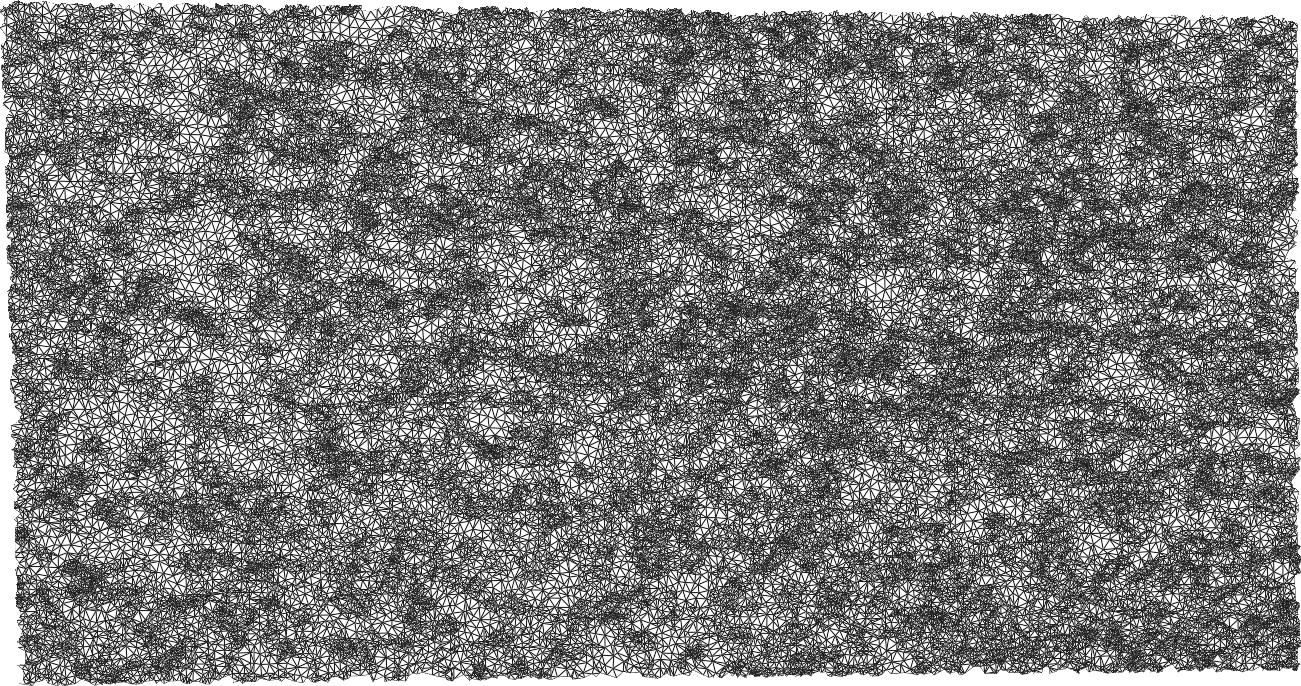
\includegraphics[width=\linewidth]
		{data/acquired_meshes/ILATO_1A_SM2066-HE5-60_070214_merged_GMO_r1_n4_v256_wireframe.png}
		\caption{wireframe}\label{ILATO:bun.a}
	\end{subfigure}
	\begin{subfigure}[b]{0.49\linewidth}
		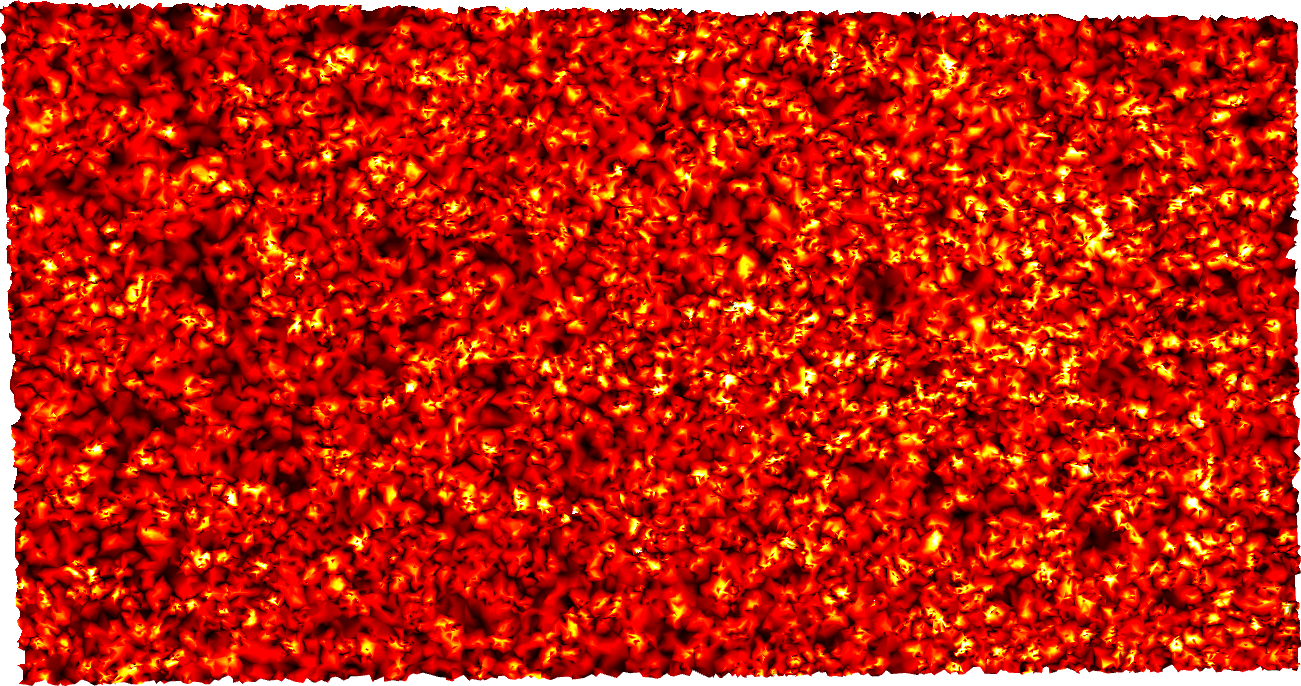
\includegraphics[width=\linewidth]
		{data/acquired_meshes/ILATO_1A_SM2066-HE5-60_070214_merged_GMO_r1_n4_v256_funcvals_0iter.png}
		\caption{$c=0$}\label{fig:buILATOn.b}
	\end{subfigure}

	\bigskip
	\begin{subfigure}[b]{0.49\linewidth}
		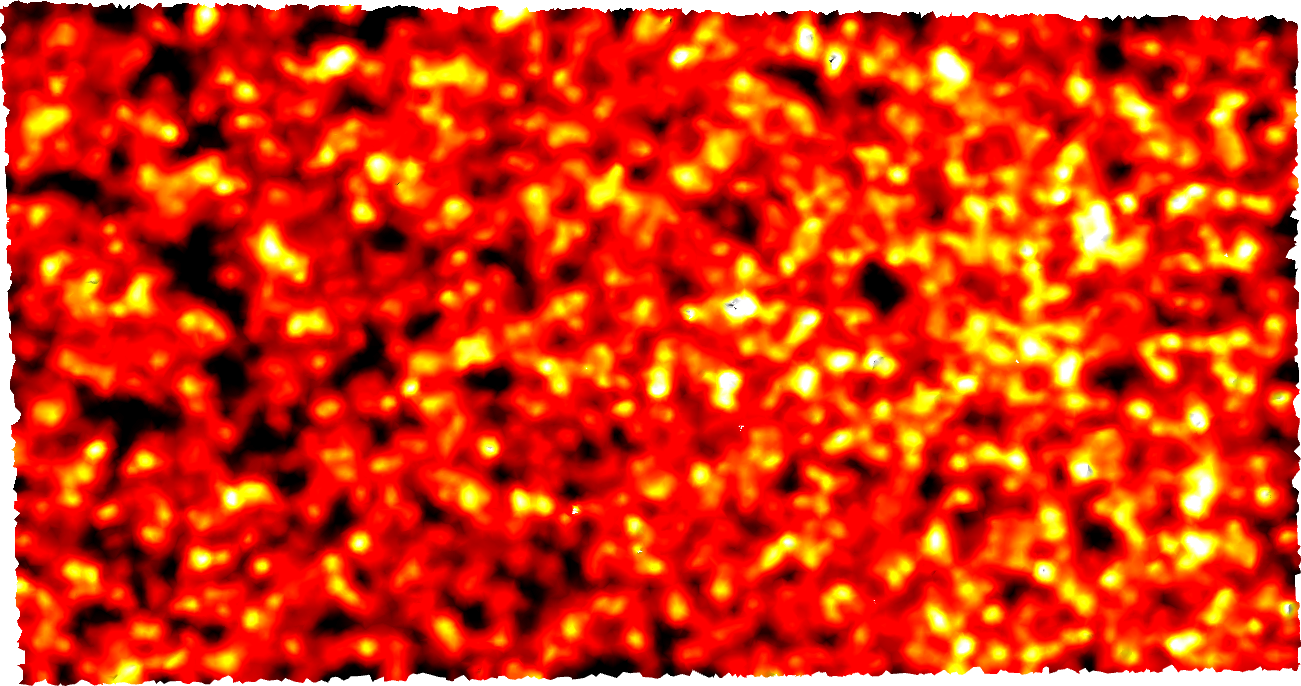
\includegraphics[width=\linewidth]
		{data/acquired_meshes/ILATO_1A_SM2066-HE5-60_070214_merged_GMO_r1_n4_v256_funcvals_1000iter.png}
		\caption{$c=1000$}\label{fig:ILATO.c}
	\end{subfigure}
	\begin{subfigure}[b]{0.49\linewidth}
		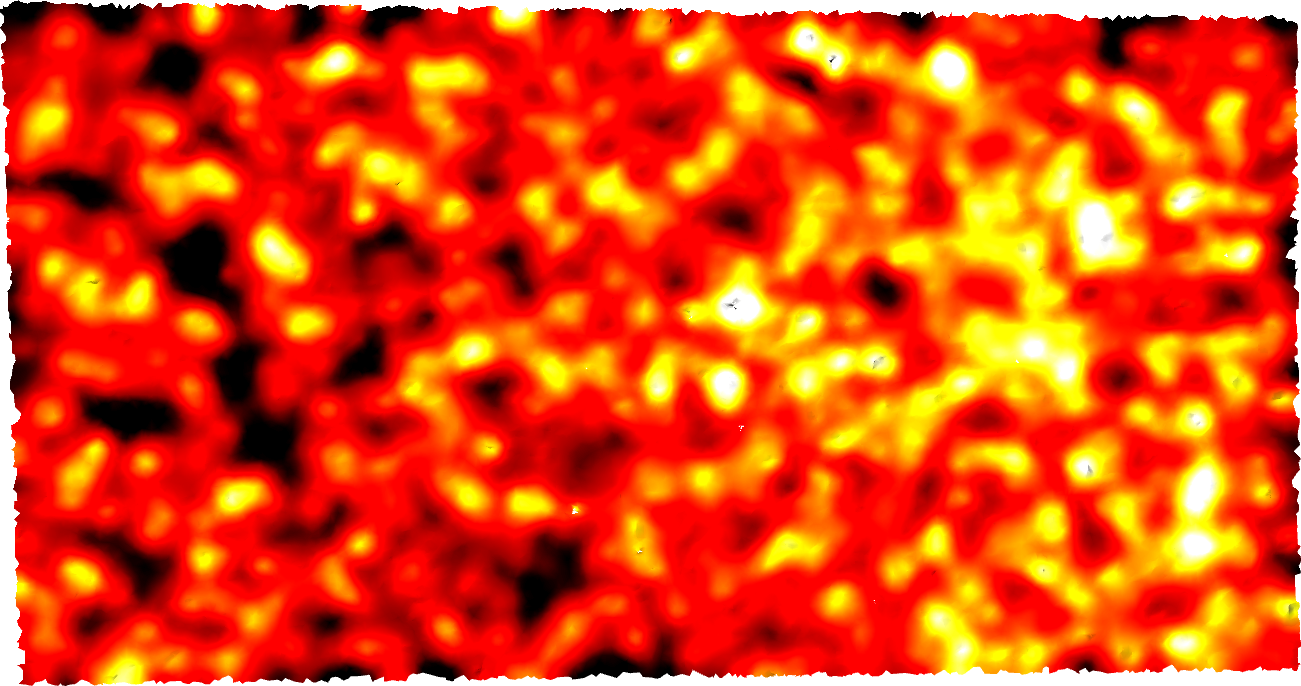
\includegraphics[width=\linewidth]
		{data/acquired_meshes/ILATO_1A_SM2066-HE5-60_070214_merged_GMO_r1_n4_v256_funcvals_3000iter.png}
		\caption{$c=3000$}\label{fig:ILATO.d}
	\end{subfigure}
	\caption[Four Views of the Flat Surface from ILATO]{Four views of a flat surface (a) in wireframe, (b) colored by \gls{tMSIIf} value before convolving the filter, (c) colored by function value after convolving the filter 1,000 times, (c) and after 3,000 times.}
	\label{fig:ILATO}
\end{figure}
